\begin{figure}[tbp]
\centering
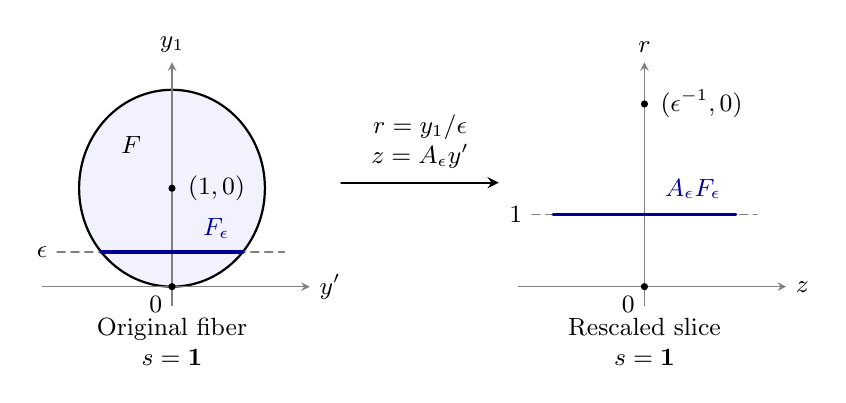
\begin{tikzpicture}[x=1cm,y=1cm,>=stealth,
  every node/.style={font=\small},line cap=round]
  \begin{scope}[shift={(0,0)}]
    \fill[blue!5] (0,1.25) ellipse[x radius=1.18,y radius=1.25];
    \draw[thick] (0,1.25) ellipse[x radius=1.18,y radius=1.25];
    \draw[->,gray] (-1.65,0)--(1.75,0) node[right,black] {$y'$};
    \draw[->,gray] (0,-.24)--(0,2.85) node[above,black] {$y_1$};
    \draw[densely dashed,gray] (-1.46,.44)--(1.43,.44);
    \draw[very thick,blue!60!black] (-.899,.44)--(.899,.44);
    \node[left] at (-1.46,.44) {$\epsilon$};
    \node[anchor=south west,blue!60!black] at (.27,.49) {$F_\epsilon$};
    \fill (0,0) circle[radius=1.3pt];
    \node[below left] at (0,0) {$0$};
    \fill (0,1.25) circle[radius=1.3pt];
    \node[anchor=west] at (.08,1.25) {$(1,0)$};
    \node at (-.52,1.8) {$F$};
    \node[align=center] at (0,-.7) {Original fiber\\$s=\mathbf1$};
  \end{scope}
  \draw[->,thick] (2.15,1.32)--(4.15,1.32);
  \node[align=center] at (3.15,1.84)
    {$r=y_1/\epsilon$\\$z=A_\epsilon y'$};
  \begin{scope}[shift={(6,0)}]
    \draw[->,gray] (-1.6,0)--(1.8,0) node[right,black] {$z$};
    \draw[->,gray] (0,-.24)--(0,2.85) node[above,black] {$r$};
    \draw[densely dashed,gray] (-1.43,.92)--(1.43,.92);
    \draw[very thick,blue!60!black] (-1.16,.92)--(1.16,.92);
    \node[left] at (-1.43,.92) {$1$};
    \node[anchor=south west,blue!60!black] at (.14,.99)
      {$A_\epsilon F_\epsilon$};
    \fill (0,0) circle[radius=1.3pt];
    \node[below left] at (0,0) {$0$};
    \fill (0,2.32) circle[radius=1.3pt];
    \node[anchor=west] at (.08,2.32) {$(\epsilon^{-1},0)$};
    \node[align=center] at (0,-.7) {Rescaled slice\\$s=\mathbf1$};
  \end{scope}
\end{tikzpicture}
\caption{The change from $(y_1,y')$ to $(r,z)$ at the fixed base
point $s=\mathbf1$, shown schematically with one $y'$ coordinate.
The actual fiber need not have the smooth or symmetric shape drawn here.
The slice $y_1=\epsilon$ becomes the slice $r=1$, while
$A_\epsilon$ normalizes its remaining transverse coordinates.
The interior point $(1,0)$ of $F$ is sent to
$(\epsilon^{-1},0)$. The right panel shows only this point, the
origin, and the distinguished slice; the shape of the transformed
fiber is omitted.}
\label{fig:thin-slice}
\end{figure}
